\section{Solidity to Control-Flow Graph}

Here we describe how we model Solidity programs as control-flow graphs. First we discuss how to model individual functions, in Section \ref{sec:sol_cfg_fun}, and then, in Section \ref{sec:sol_cfg_con}, the general approach for modelling a whole contract is presented.

%%%%%%%%%%%%%%%%%%%%%%%%%%%%%%%%%%%%%%%%%%

\subsection{Control-Flow Graph of a Solidity Function} \label{sec:sol_cfg_fun}

To generate the control-flow graph of a Solidity function we initially create an entry node to represent its start. Beginning from the entry node, the code is scanned until the function ends or a return statement is reached. During the scanning process, statements that do not influence the control-flow, such as assignments, are stored in the current node for future analysis. When control structures are reached, however, the graph is updated according to their semantics. To model the end of the function, a sink, called the exit node, is created, being the targeted by every node with a return statements, and if none exist, by node storing the last statement of the function.

The shape of the resulting graph depends of the control structures present in the function. The graphs generate by some common structures can be seen inside the dotted squares in figures \ref{fig:cfg_if}, \ref{fig:cfg_if-else}, and \ref{fig:cfg_while}; the edges with no tag have value \texttt{true}. Each condition generates an empty node with two outward edges, one with the condition itself, and one with its negation. Control structures can be combined to model complex scenarios, such as nested loops.

The encoding of the Solidity assertions is done according to their semantics. The \texttt{require} operator works as a pre-condition, and is thus simply added inside the current node. The \texttt{assert} operator works as a post-condition, and is encoded as a conditional with the \texttt{then} branch targeting the next node in the graph, and the \texttt{else} branch targeting the error node. The error node is a special sink node in our model, and reaching it represents an error in the execution. The graph representing an \texttt{assert} can be seen in Figure \ref{fig:cfg_assert}.

\begin{figure}[ht]
  \centering
  \begin{minipage}[h]{0.43\textwidth}
  	\centering
    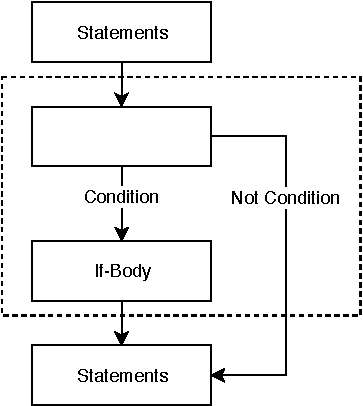
\includegraphics[width=0.6\textwidth]{images/if}
    \caption{Graph of the if-then}
    \label{fig:cfg_if}
  \end{minipage}
  \begin{minipage}[h]{0.43\textwidth}
  	\centering
    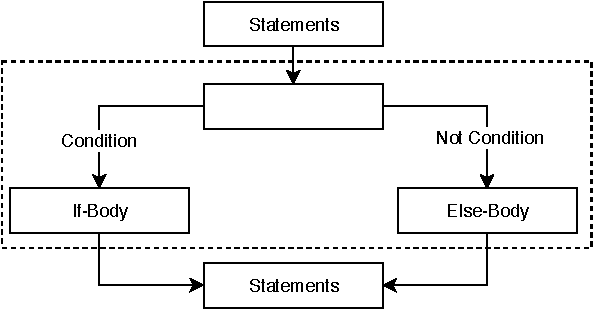
\includegraphics[width=\textwidth]{images/if-else}
    \caption{Graph of the if-then-else}
    \label{fig:cfg_if-else}
  \end{minipage}
  \newline \newline \vfill
  \begin{minipage}[h]{0.43\textwidth}
  	\centering
    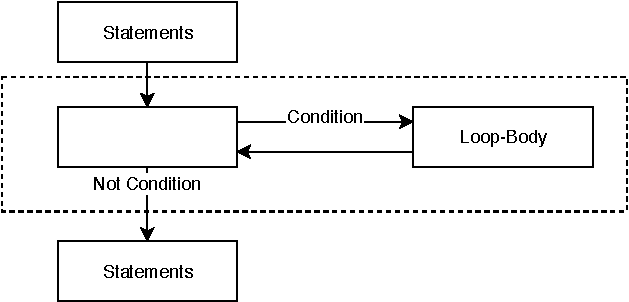
\includegraphics[width=\textwidth]{images/while}
    \caption{Graph of the while-loop}
    \label{fig:cfg_while}
  \end{minipage}
  \begin{minipage}[h]{0.43\textwidth}
  	\centering
    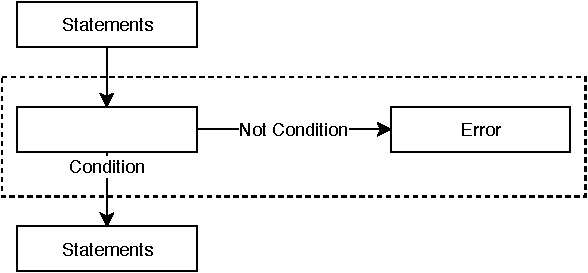
\includegraphics[width=\textwidth]{images/assert}
    \caption{Graph of the assert}
    \label{fig:cfg_assert}
  \end{minipage}
\end{figure}

Function calls, be them  recursive calls, calls to functions in the same contract or in another contract, are always considered to be inlined. The source code of all functions called is thus required for the generation of the control-flow graph.

The control-flow graph of \texttt{average} function shown in Section \ref{sec:background_sol} can be seen in Figure \ref{fig:cfg_average}. In this example we can see that the variables \texttt{count} and \texttt{sum} are used but not defined, since they are state variables; the return variable is initialized with its default value. To correctly encode state variables, a model of the whole contract is required.

\begin{figure}[ht]
	\centering
	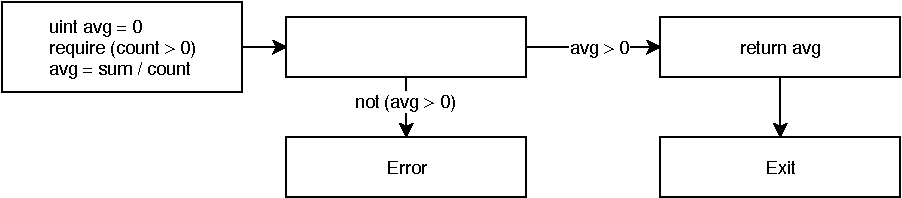
\includegraphics[width=0.7\textwidth]{images/average}
	\caption{Graph of the \texttt{average} function}
	\label{fig:cfg_average}
\end{figure}

%%%%%%%%%%%%%%%%%%%%%%%%%%%%%%%%%%%%%%%%%%

\subsection{Control-Flow Graph of a Solidity Contract} \label{sec:sol_cfg_con}

Solidity contracts do not have a main function, once deployed to the blockchain all their functions, with the appropriate visibility, can be called many times and in any order. To capture this behaviour in a single control-flow graph, we create an infrastructure to model calls to functions, as can be seen in Figure \ref{fig:cfg_contract-general}.

\begin{figure}[ht]
	\centering
	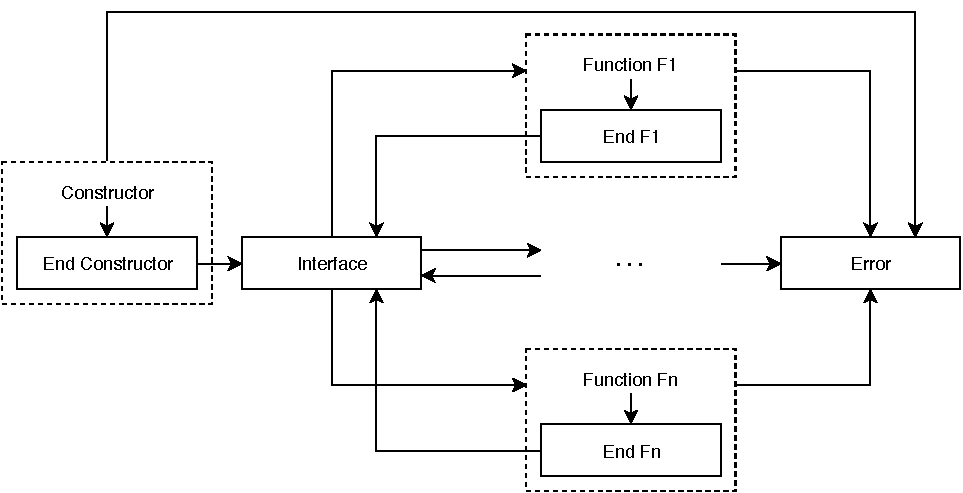
\includegraphics[width=0.7\textwidth]{images/contract-general}
	\caption{Graph of a Solidity contract}
	\label{fig:cfg_contract-general}
\end{figure}

The entry node of the graph is the constructor of the contract, which is a special function that is executed before deploying the contract on the blockchain, with the goal of initializing state variables. After the constructor we have the interface node, which is an empty node that targets the entry of each function in the contract. To represent the nondeterminism in the order in which the functions are called, all transitions starting at the interface have value \texttt{true}. Multiple function calls are enabled through the edges between the exits nodes of each function and the interface. To simplify the analysis, the contract model has a single error state instead of one for each function. 

The graph that models the contract \texttt{C}, shown in Section \ref{sec:background_sol}, can be seen in Figure \ref{fig:cfg_contract-c}. Due to absence of \texttt{assert} statements in the constructor and the fallback function, there is only one edge targeting the error node, starting from the \texttt{average} function. Every function that is \texttt{payable}, such as the fallback function in our example, has a \texttt{msg} object implicitly defined, with \texttt{msg.value} being the amount of ether sent to the function. Since the state of \texttt{msg} depends on the arguments of the call, \texttt{msg.value} is initialized with a nondeterministic value, symbolised by \texttt{\#}.

\begin{figure}[ht]
	\centering
	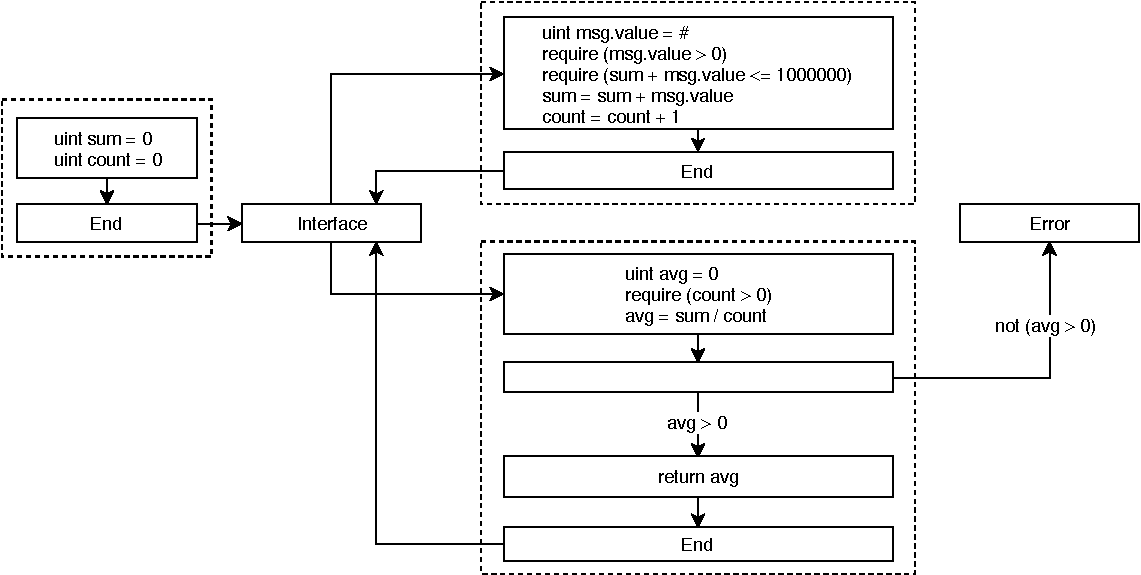
\includegraphics[width=0.85\textwidth]{images/contract-c}
	\caption{Graph of the \texttt{C} contract}
	\label{fig:cfg_contract-c}
\end{figure}
